\chapter{Livello fisico}

Come riportato nella sezione~\ref{ss:dw-phy}, l'interfaccia tra debug server, l'ATMega16U2, e il controllore target è costituita da una linea seriale open drain.

Si rende necessario quindi implementare tale interfaccia in modo efficiente al fine di permettere al server GDB di interfacciarsi con il \textit{target} tramite DebugWire

\section{Implementazione}

\subsection{Implementazione ideale}
L'implementazione inizialmente progettata in fase di ideazione, ancora prima che fosse stabilita la piattaforma hardware, sfruttava la periferica UART presente sul controllore ATMega16U2\cite[chap. 18]{avr:m16u2}.

Al fine di implementare l'accesso alla linea open drain si rende necessario l'utilizzo di un componente aggiuntivo come mostrato nella figura~\ref{fig:od-impl}, la quale mostra due alternative di implementazione utilizzando un diodo o un transistor. 

\begin{figure}[t]
    \centering

    \subfloat[][]{
        \begin{circuitikz}
            \draw (0, 0) node[label={[font=\footnotesize]above:rxd}] {} to[short, *-] (2, 0) to[short, -] (2, 1) to[R={\(R_{pullup}\)}] (2, 2) to [short, -] (2, 2.5) to [short, -] (2.5, 2.5) to [short, -] (2.5, 3);
            \draw (2.5, 2.5) to[short, -] (3, 2.5) to[short, -] (3, 2) to[R={\(R1\)}] (3, 1);
            \draw (3,-1) node [npn,xscale=-1,anchor=B] (npn) {} (npn.collector);
            \draw (3, 1) to[short, -] (3, -1);
            \draw (2, 0) to[short, *-*] (4, 0) node[label={[font=\footnotesize]above:target}] {};
            \draw (0, -2) node[label={[font=\footnotesize]above:txd}] {} to[short, *-]  (2.16, -2) to[short, -] (2.16, -1.75);
            \draw (2.16, 0) to[short, *-] (2.16, -0.5);
            \draw (2, 3) -- node[anchor=south,align=center] {VCC} (3, 3);
        \end{circuitikz}
    }
    \subfloat[][]{
        \begin{circuitikz}
            \draw (0, 0) node[label={[font=\footnotesize]above:rxd}] {} to[short, *-] (2, 0) to[short, -] (2, 1) to[R={\(R_{pullup}\)}] (2, 2) to [short, -] (2, 3);
            \draw (1.5, 3) -- node[anchor=south,align=center] {VCC} (2.5, 3);
            \draw (2, 0) to[short, *-*] (4, 0) node[label={[font=\footnotesize]above:target}] {};
            \draw (2, 0) to[short, -] (2, -0.5) to[D={\(D1\)}] (2, -1.5) to[short, -] (2, -2)  to [short, -*] (0, -2) node[label={[font=\footnotesize]above:txd}] {};
        \end{circuitikz}
    }
    \caption[]{L'immagine mostra due possibili circuiti per l'adattamento della periferica UART dell'ATMega16U2 alla linea seriale open drain.}\label{fig:od-impl}
\end{figure}

Il principio di funzionamento dei circuiti in figura~\ref{fig:od-impl} è pressoché identico: Il valore del pin txd viene replicato sulla linea di connessione con un livello logico 0 ``forte'' e un livello logico 0 ``debole'' dato dalla resistenza \(R_{pullap}\) e in entrambi i casi il pin txd viene utilizzato come collettore di corrente.
La differenza consiste nella quantità di componenti aggiuntivi e nelle prestazioni.

Il circuito (a) consente di raggiungere un livello logico 0 pari a circa 0.3V, data dalla differenza di potenziale \(V_{ce}\) del transistor in saturazione, mentre il circuito (b) raggiunge un livello logico 0 di 0.7V data dalla caduta di tensione del diodo. Nel secondo caso sarebbe possibile migliorare le prestazioni utilizzano un diodo \textit{schottky} causando però un innalzamento della capacitanza della linea.

I risultati sopra mostrati sono verificati dalle simulazioni i cui risultati sono mostrati in figura~\ref{graph:sim}.

\begin{figure}
    \centering
        \begin{tikzpicture}
            \begin{axis}[
                width=0.8\textwidth,
                xlabel={Tempo (S)},
                ylabel={Tensione (V)}
                ]
                \addplot table [x=t, y=v(tgt), col sep=comma, mark=none] {sims/phy-sim-bjt.csv};
                \addplot table [x=t, y=v(txd), col sep=comma, mark=none] {sims/phy-sim-bjt.csv};
                \legend{$tgt$,$txd$}
            \end{axis}
        \end{tikzpicture}\\
        \vfill
        \begin{tikzpicture}
            \begin{axis}[
                width=0.8\textwidth,
                xlabel={Tempo (S)},
                ylabel={Tensione (V)}
                ]
                \addplot table [x=t, y=v(tgt), col sep=comma, mark=none] {sims/phy-sim-diode.csv};
                \addplot table [x=t, y=v(txd), col sep=comma, mark=none] {sims/phy-sim-diode.csv};
                \legend{$tgt$,$txd$}
            \end{axis}
        \end{tikzpicture}
    \caption[]{Risultati della simulazione dei circuiti in figura~\ref{fig:od-impl} con tempo di bit pari a 8\(\mu\)S}\label{graph:sim}
\end{figure}

Come è possibile notare nel secondo caso la tensione della linea \textit{tgt} non è mai inferiore a 0.7V.

Sfruttando la periferica UART dell'ATMega16U2 risulta quindi notevolmente semplificata l'implementazione della comunicazione DebugWire, oltre a rendere possibile un approccio ad interrupt per la scrittura del firmware.

\subsection{Implementazione effettiva}

Data la scelta di riutilizzare modificando la scheda \textit{Arduino UNO R3}, si è reso necessario l'utilizzo di un solo pin (pin 13) in quanto già collegato al pin di reset dopo le modifiche apportate descritte dalla sezione~\ref{s:dw-board-mod}.

Di conseguenza si è reso necessario scrivere un'implementazione software del protocollo seriale tramite un solo pin.

La prima difficoltà di impleentazione riguarda la gestione del pin per l'utilizzo OpenDrain: la piattaforma AVR non supporta nativamente in hardware tale funzione, rendendo necessaria la gestione dello stato del pin a livello software.

Vi sono tre registri di gesione di un pin nell'architettura AVR:\ \texttt{PORTx, DDRx e PINx}. A ogni bit di questi registri è associato un pin fisico e il relativo stato.

Attraverso quanto è rappresentato nella figura~\ref{fig:avr-pin} possiamo valutare le varie condizioni nelle quali il pin fisico può trovarsi in funzione dello stato dei bit relativi ai tre registri elencati in precedenza.

\begin{figure}[t]
    \centering
    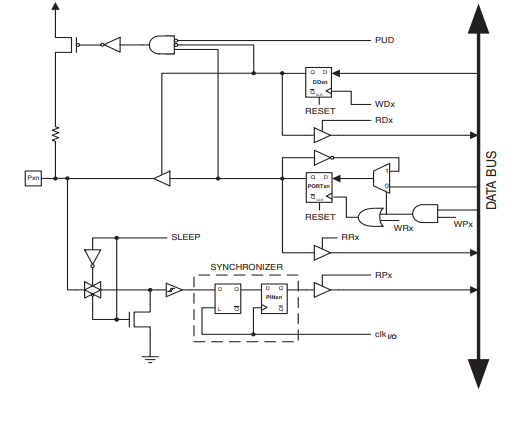
\includegraphics[width=.85\textwidth]{avr-pin-diag.png}
    \caption[Immagine ottenuta dal documento\cite{avr:m16u2}, fig. 12-2]{Diagramma funzionale dell'hardware relativo a un generico pin della famiglia AVR\cite[fig. 12-2]{avr:m16u2}}\label{fig:avr-pin}
\end{figure}

Alla scrittura del registro DDRx viene asserita la linea WDx, la quale salva lo stato del bit associato al pin nel flipflop pilotato da essa. Questo stato pilota un buffer che stabilisce se il pin stesso debba essere un input o un output.

In particolare, se lo stato salvato nel primo flipflop è 1, il pin sarà pilotato con livello logico pari allo stato salvato nel secondo flipflop in modo ``forte''.

Se invece lo stato del pin viene posto come input, ossia lo stato del primo flipflop è 0, è possibile pilotare il FET che alimenta la linea di pullup del pin. Questo accade perchè il segnale che rappresenta la direzione del pin è input negato della porta AND che controlla lo stato del pullup; per questo motivo, lo stato 0 permette alla porta di avere risultato 1 se lo stato del secondo flipflop è pari a 1, in quanto tale segnale sarebbe ignorato perchè il buffer di controllo è disabilitato.

La lettura dello stato del pin può avvenire in qualunque momento tramite la lettura del registro PINx, il quale asserisce la linea RPx e riporta lo stato salvato nello stadio di sincronizzazione.

La scrittura di tale registro viene reindirizzata al controllo del multiplexer in modo da poter invertire lo stato del pin senza averlo precedentemente letto, dimezzando la quantità di operazioni necessarie.




%usando un solo pin
%state machine?
